\documentclass[a4paper,12pt]{extarticle}

\usepackage[T1]{fontenc}
\usepackage[utf8]{inputenc}

\usepackage[]{parskip}
\usepackage{hyperref, wrapfig, float, amsmath, adjustbox, array, pdflscape, soul, color, extsizes}

\renewcommand{\arraystretch}{2}
\renewcommand{\contentsname}{Spis treści}
\renewcommand{\refname}{Bibliografia}
\renewcommand{\figurename}{Rys.}
\renewcommand{\tablename}{Tab.}

\usepackage{geometry}
\geometry{
  a4paper,
  margin=20mm,
  bottom=30mm
}

\usepackage{graphicx}
\usepackage{caption}
\usepackage{subcaption}
\usepackage[font=small,labelfont=bf]{caption}
\graphicspath{ {./images/}{../images/} }

\newcommand{\mathcolorbox}[1]{
  \begin{center}
    \colorbox{yellow}{$\displaystyle #1$}
  \end{center}
}
\newcommand{\pvec}[1]{
  \vec{#1}\mkern2mu\vphantom{#1}
}
\newcommand{\angstrom}{\mbox{\normalfont\AA}}

\begin{document}
  \begin{titlepage}
    \begin{center}
      \begin{figure}[H]
        \centering
        
\includegraphics[scale=.125]{logopp.png}
      \end{figure}
      \vspace*{.05\textheight}
      \huge\textbf{Politechnika Poznańska}\\
      \large\textbf{Wydział Inżynierii Materiałowej i Fizyki Technicznej}\\
      \large\textbf{Fizyka Techniczna}\\
      \vspace*{.2\textheight}
      \huge\textbf{Modelowanie cząsteczki wody}\\
      \vspace*{.025\textheight}
      \large\textbf{Jakub Bąbelek\\(nr.\ albumu: 136454)}
    \end{center}
  \end{titlepage}

  \tableofcontents
  
  \clearpage
  \section{Wstęp}
  Woda ($H_2O$) jest jedną z najpowszechniejszych substancji na ziemi. Jej molekułę
  tworzą 2 atomy wodoru i atomu tlenu które razem tworzą tetraedr w którym atom
  tlenu zajmuje miejsce w środku. Wiązania cząsteczki wody są silnie spolaryzowane
  przez co jest ona silnie polarna oraz jest dipolem,
  może wykonywać ruchy translacyjne, oscylacyjne jak i rotacyjne. W warunkach
  standardowych jest bezwonną, bezbarwną cieczą.

  \noindent Właściwości fizyczne cząsteczki:
  \begin{itemize}
    \item{Długość wiązania: \( 1,013 \angstrom \)}
    \item{Kąt: \(104^o27'\)}
    \item{Ciepło tworzenia: \( -68.2694 \dfrac{kcal}{mol} \)}
    \item{Moment dipolowy: \( 1,8546 \pm 0,0040 D \)}
  \end{itemize}

  \noindent Do modelowania molekuły wody użyliśmy 4 metod:
  \begin{enumerate}
    \item
    UFF (Universal Force Field) - Metoda klasyczna, niewykorzystująca elmentów fizyki kwantowej.
    
    \item
    AM1 (Austin Model  1) - Półempiryczna metoda kwantowa służąca do obliczeń struktury elektronwej.
    Głównym jej założeniem jest formalizm Hartee-Focka.
    
    \item
    PM3 (Parametric Model 3) - Półempiryczna metoda kwantowa służąca do obliczeń struktury elektronwej.
    Metoda podobna do AM1 lecz używająca innych wartości parametrów formalizmu Hartee-Focka.
    
    \item
    DFT (Density Funcional Theory) - Kwantowa metoda służąca do obliczeń struktury elektronwej.
    Dzięki zastosowaniu funkcjonału gęstości stanów elektronowych
    tą metodą jesteśmy w stanie uzyskać właściwości układów wieloelektronowych.
  \end{enumerate}

  \clearpage
  \section{Wyniki}

  Rys. \ref{fig:h2o} przedstawia wstępny model stworzony w programie ArgusLab. Geometria
  cząsteczki jest jedynie poglądowa.

  \begin{figure}[H]
    \centering
    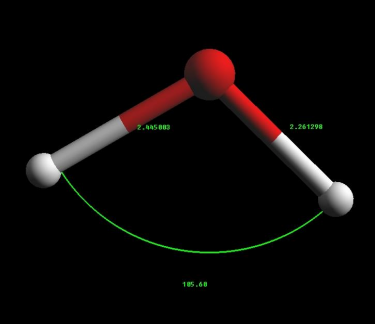
\includegraphics[scale=1]{h2o.png}
    \caption{Cząsteczka przed optymalizacją}
    \label{fig:h2o}
  \end{figure}

  Rys. \ref{fig:h2o_uff} to cząsteczka po optymalizacji metodą UFF. Porównując
  wyniki z wartościami rzeczywistymi widzimy, że nie jest ona dokładna lecz pozwala
  w prosty sposób uzyskać obraz molekuły zbliżony do rzeczywistego.

  \begin{figure}[H]
    \centering
    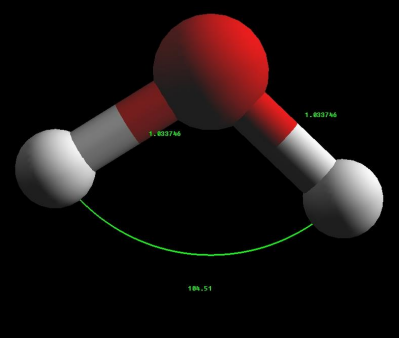
\includegraphics[scale=1]{h2o_uff.png}
    \caption{Cząsteczka po użyciu metody UFF}
    \label{fig:h2o_uff}
  \end{figure}

  Rys. \ref{fig:h2o_am1} ukazuje molekułę zoptymalizowaną metodą AM1. Jest to wynik
  najbliższy rzeczywistemu, widać znaczącą poprawę w dokładności długości wiązań i
  kąta między nimi.

  \begin{figure}[H]
    \centering
    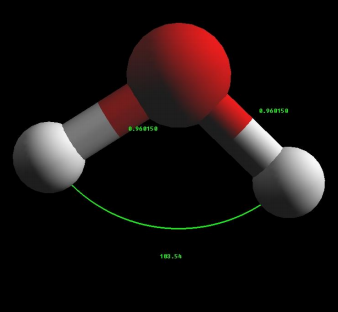
\includegraphics[scale=1]{h2o_am1.png}
    \caption{Cząsteczka po użyciu metody AM1}
    \label{fig:h2o_am1}
  \end{figure}

  Tabela \ref{tab:wyniki} przedstawia zestawienie użytych metod.

  \begin{table}[h]
    \begin{adjustbox}{max width = \textwidth}
      \begin{tabular}{c|c|c|c|c|c}
      \textbf{Metoda} & \textbf{Długość wiązania \( [\angstrom] \)} & \textbf{Kąt \( [^o] \)} & \textbf{\begin{tabular}[c]{@{}c@{}}Energia całkowita\\ termodynamiczna\\ \( \left[\dfrac{kcal}{mol}\right] \)\end{tabular}} & \textbf{Ciepło tworzenia \( \left[\dfrac{kcal}{mol}\right] \)} & \textbf{Moment dipolowy \( [D] \)} \\ \hline
      UFF             & 1,033746                                    & 104,51                  & 0                                                                                                                           & -                                                              & -                                  \\
      AM1             & 0,960150                                    & 103,54                  & -8036,9395                                                                                                                  & -58,3019                                                       & 1,85911636                         \\
      PM3             & 0,952968                                    & 107,59                  & -7490,3948                                                                                                                  & -51,4437                                                       & 1,74037872                         \\
      DFT             & 1,0855                                      & 96,746                  & -11310,2598                                                                                                                 & -                                                              & -                                 
      \end{tabular}
    \end{adjustbox}
    \caption{Wyniki przedstawiające wszystkie użyte metody}
    \label{tab:wyniki}
  \end{table}

  \begin{figure}[H]
    \centering
    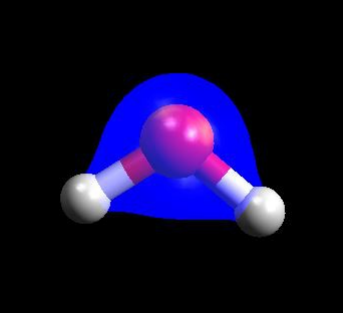
\includegraphics[scale=.8]{h2o_cont.png}
    \caption{Kontur gęstości elektronowej}
    \label{fig:h2o_am1}
  \end{figure}

  \begin{figure}[H]
    \centering
    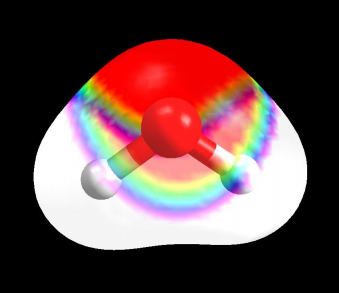
\includegraphics[scale=.8]{h2o_poten.png}
    \caption{Mapa potencjału elektrostatycznego na powierzchni gęstości elektronowej}
    \label{fig:h2o_am1}
  \end{figure}

  \subsection{Orbitale molekularne - AM1}
  
  \begin{figure}[H]
    \begin{minipage}{0.5\textwidth}%
        \centering
        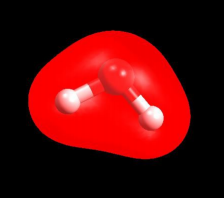
\includegraphics[scale=1]{am1_01.png}
        \caption{O 2S (wiążący)}
        \label{fig:am1_01}
    \end{minipage}%
    \begin{minipage}{0.5\textwidth}%
        \centering
        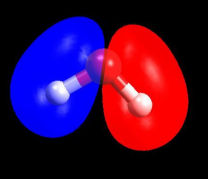
\includegraphics[scale=1]{am1_02.png}
        \caption{O 2Px (wiążący)}
        \label{fig:am1_02}
    \end{minipage}
  
    \begin{minipage}{0.5\textwidth}%
        \centering
        \captionsetup{justification=centering}
        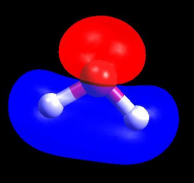
\includegraphics[scale=1]{am1_03.png}
        \caption{O 2Py (wiążący)}
        \label{fig:am1_03}
    \end{minipage}%
    \begin{minipage}{0.5\textwidth}%
        \centering
        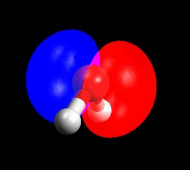
\includegraphics[scale=1]{am1_04.png}
        \caption{O 2Pz (wiążący)}
        \label{fig:am1_04}
    \end{minipage}

    \begin{minipage}{0.5\textwidth}%
        \centering
        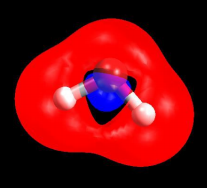
\includegraphics[scale=1]{am1_05.png}
        \caption{H 1S (niewiążący)}
        \label{fig:am1_05}
    \end{minipage}%
    \begin{minipage}{0.5\textwidth}%
        \centering
        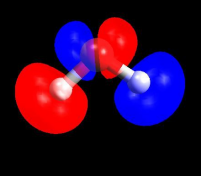
\includegraphics[scale=1]{am1_06.png}
        \caption{H 1S (niewiążący)}
        \label{fig:am1_06}
    \end{minipage}
  \end{figure}

  \subsection{Orbitale molekularne - PM3}

  \begin{figure}[H]
    \begin{minipage}{0.5\textwidth}%
        \centering
        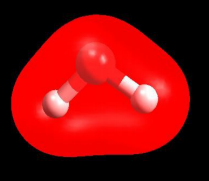
\includegraphics[scale=1]{pm3_01.png}
        \caption{O 2S (wiążący)}
        \label{fig:pm3_01}
    \end{minipage}%
    \begin{minipage}{0.5\textwidth}%
        \centering
        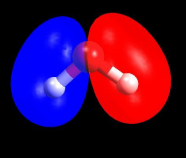
\includegraphics[scale=1]{pm3_02.png}
        \caption{O 2Px (wiążący)}
        \label{fig:pm3_02}
    \end{minipage}
  
    \begin{minipage}{0.5\textwidth}%
        \centering
        \captionsetup{justification=centering}
        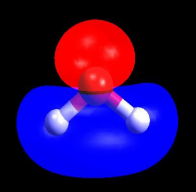
\includegraphics[scale=1]{pm3_03.png}
        \caption{O 2Py (wiążący)}
        \label{fig:pm3_03}
    \end{minipage}%
    \begin{minipage}{0.5\textwidth}%
        \centering
        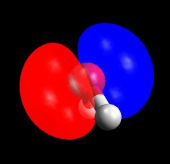
\includegraphics[scale=1]{pm3_04.png}
        \caption{O 2Pz (wiążący)}
        \label{fig:pm3_04}
    \end{minipage}

    \begin{minipage}{0.5\textwidth}%
        \centering
        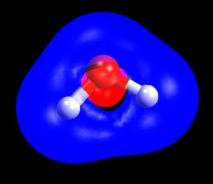
\includegraphics[scale=1]{pm3_05.png}
        \caption{H 1S (niewiążący)}
        \label{fig:pm3_05}
    \end{minipage}%
    \begin{minipage}{0.5\textwidth}%
        \centering
        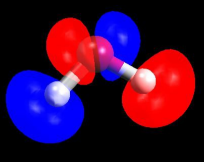
\includegraphics[scale=1]{pm3_06.png}
        \caption{H 1S (niewiążący)}
        \label{fig:pm3_06}
    \end{minipage}
  \end{figure}

  \clearpage
  \begin{thebibliography}{9}
    \addcontentsline{toc}{section}{Bibliografia}
        
    \bibitem{arguslab}
    Obliczenia i wizualizacje zostały wykonane za pomocą:\\
    \textit{ArgusLab 4.0}\\
    Mark A. Thompson\\
    Planaria Software LLC, Seattle, WA.
    http://www.arguslab.com
  \end{thebibliography}

\end{document}